\rhead{相关概念与相关工作介绍}
\chapter{相关概念与相关工作介绍}

%@@@@@@@@@@@@@@@@@@@@@@@@@@@@@@@@@@
\section{相关概念介绍}
本节主要对本文中经常出现的一些概念作相关介绍以及形式化的定义。

\subsection{PPI网络}
蛋白质相互作用网络(protein-protein interaction networks),简称PPI网络,是一种生物体内表示蛋白质相互之间作用的模型。定义图$G=(V,E)$为一个PPI网络,其中$V$是点集,其中每个点代表一种蛋白质,$E$是一个$V×V$的边集,一条边$(u,v)$代表蛋白质$u$和$v$具有相互作用。由定义可知$G$是一个无权无向图。
%@@@@@@@@@@@@@@@@@@@@@@@@@@@@@@@@@@@@@@@@@@@@@@@@
\subsection{全局网络匹配}
全局网络匹配(global networks alignment)是对两个PPI网络$G_1(V_1,E_1)$,$G_2(V_2,E_2)$进行匹配的过程,不失一般性,$|V_1|\leq|V_2|$,并且称$G_1$为源网络(source network),$G_2$为目标网络(target network)。匹配的结果是一个从$V_1$到$V_2$的单射$f:V_1\rightarrow V_2$。因此在全局网络匹配中,$G_1$的每个点都对应$G_2$中不同的点,令$v_1\in V_1$为图$G_1$中的一个点,则$f(v_1)\in V_2$则是$v_1$在$G_2$中对应的匹配点。

在匹配$f$下,如果有一条源网络中的边$(u,v)\in E_1$满足$(f(u),f(v))\in E_2$,则称边$(u,v)$在$f$下是被保留(匹配)的边。

令$X\subseteq V$,则$G[X]$表示图$G$中点集$X$的导出子图(induced subgraph),且$E(G[X])$表示该导出子图的边集合。令$f(E_1)=\left \{(f(u),f(v))\in E_2:(u,v)\in E_1\right \}$,并且令$f(V_1)=\left\{f(v)\in V_2:v\in V_1\right\}$。

如何衡量一个匹配的好坏,是网络匹配中一个重要的问题,因此存在许多种不同的衡量指标(alignment quality measure)。
$$EC(f)=\frac{\left | f(E_1) \right |}{\left | E_1 \right |}\cite{kuchaiev2010topological}$$表示被匹配的边数占源网络总边数的比例,是最为常见的衡量指标。但是由于是对比源网络的边,在源网络是稀疏网络,目标网络是稠密网络的情况下,该指标并不能很好的衡量匹配效果。
$$ICS(f)=\frac{\left | f(E_1) \right |}{\left |E_2(G_2[f(V_1)])\right |}\cite{patro2012global}$$则表示被匹配的边数在目标网络中被匹配的点集所引出的导出子图中所占的边数比例,与$EC$指标恰好相反,该指标在源网络是稠密网络,目标网络是稀疏网络的时候,不能体现很好的效果。
$$TWEC(f)=\frac{EC(f)+ICS(f)}{2}\cite{dopmann2013survey}$$则平均了上面两个指标,一定程度上缓解了极端情况下衡量效果不好的情况。
$$S^{3}(f)=\frac{\left | f(E_1) \right |}{\left | E_1 \right |+\left | E_2(G_2[f(V_1)]) \right |-\left | f(E_1) \right |}\cite{saraph2014magna}$$则同时考虑了源网络和目的网络,相对$EC$和$ICS$来说是一个更值得考量的指标。

\begin{figure}[htbp]
\centering
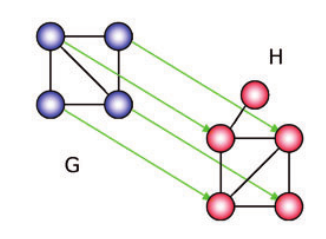
\includegraphics[height=0.25\textheight]{pic/measure.png}
\captionsetup{margin=50pt}
\caption{$G$为源网络,$H$为目标网络,其中各项指标的值分别为$EC=4/5=0.8,ICS=4/5=0.8,TWEC=0.8,S^3=4/6=0.67$ \cite{saraph2014magna} \label{fig:measure}}
\end{figure}

%@@@@@@@@@@@@@@@@@@@@@@@@@@@@@@@@@@@
\section{相关工作介绍}
关于PPI网络的全局匹配算法,到目前为止非常的多,本文主要对其中四种经典的算法进行简单的介绍。
%@@@@@@@@@@@@@@@@@@@@@@@@@@@@@@@@@@@@@@@@
\subsection{IsoRank算法}
IsoRank是全局网络匹配问题中被提出的第一个具有开拓性意义的算法。它主要分为两步。
第一步,IsoRank算法计算源网络$G_1$和目标网络$G_2$之间任意点对之间的相似性,用一个分数$R_{ij},i\in V_1,j\in V_2$来表示。IsoRank算法借鉴了Google的PageRank算法,任意点对$(i,j)$之间的价值由$i$和$j$两个点的邻居节点的价值所决定。

\begin{equation}\label{isorank1}
R=\sum R_{ij}=\sum_{u\in N(i),v\in N(j)}\frac{1}{\left | N(u) \right |\left | N(v) \right |}R_{uv}
\end{equation}
$N(i),N(j)$分别对应点i和点j的邻居点集。定义

\begin{equation}\label{isorank2}
A[i,j][u,v]=\begin{cases}
\frac{1}{\left | N(u) \right |\left | N(v) \right |} & \text{  } (i,u)\in E_1, (j,v)\in E_2 \\ 
 0& \text{  } \text{其他}
\end{cases}
\end{equation}
则有
\begin{equation}\label{isorank3}
R=AR
\end{equation}
从\ref{isorank3}可以看出,$R$是关于矩阵$A$的一个特征向量,在$A$是个稀疏矩阵的情况下,求解$A$的特征向量可以通过一种叫幂法(power method)的方法来迭代算出$R$,具体过程为:先随意初始化$R$,然后不断迭代,假设第$k$轮已经迭代完成,现在要进行第$k+1$轮迭代,则
\begin{equation}\label{isorank3}
R(k+1)\leftarrow AR(k)/\left \|AR(k)\right \|
\end{equation}
当$\left \|R(k+1)-R(k)\right \|\rightarrow 0$时即可终止迭代。
有了$R$,IsoRank第二步就是不断按分数从大到小挑选点对$(i,j)$,如果当前$i$和$j$都没有被匹配过,则将点对$(i,j)$加入最终的匹配结果,直到不能挑出符合条件的点对。
IsoRank可以说是全局网络匹配中第一个经典的算法,其经典之处在于其两步走的解决问题的方法。第一步定义点对之间的相似度,第二步根据相似度按某种策略产生匹配,这一解决问题的框架为之后不少提出的全局网络匹配算法所采用。
%@@@@@@@@@@@@@@@@@@@@@@@@@@@@@@@@@@@@@@@@@@@@@@@@@@@
\subsection{GRAAL算法}
GRAAL算法(GRAph ALigner)是一系列算法的总称,第一个提出的算法为GRAAL\cite{kuchaiev2010topological},而最近刚提出的算法为L-GRAAL\cite{malod2015graal}。这一系列算法的特征是都运用了一种叫小图度数(graphlet degree)的特征作为网络中一个点的拓扑结构的衡量标准。一个度数为$n$的小图(graphlet)就是一个有$n$个点的连通图(connected graph)。

图\ref{fig:graphlet}展示了所有点数在5以内的小图,可以看到这些小图的某些点被标了号,这些被标号的点被称为orbit,它们是小图中互相不同构的点。而对图$G$中的一个点$v$,其所谓的节点小图度数,是一个向量,其中向量的第$i$维表示的值就是以点$v$为中心,第$i$个orbit代表的小图出现的次数,形象化理解,就是将点$v$与第$i$个orbit匹配,看第$i$个orbit所在的小图是否能够匹配上以点$v$为中心延伸出去的子图,不同的子图分别计数,总出现次数就是第$i$维所表示的值。


\begin{figure}[htbp]
\centering
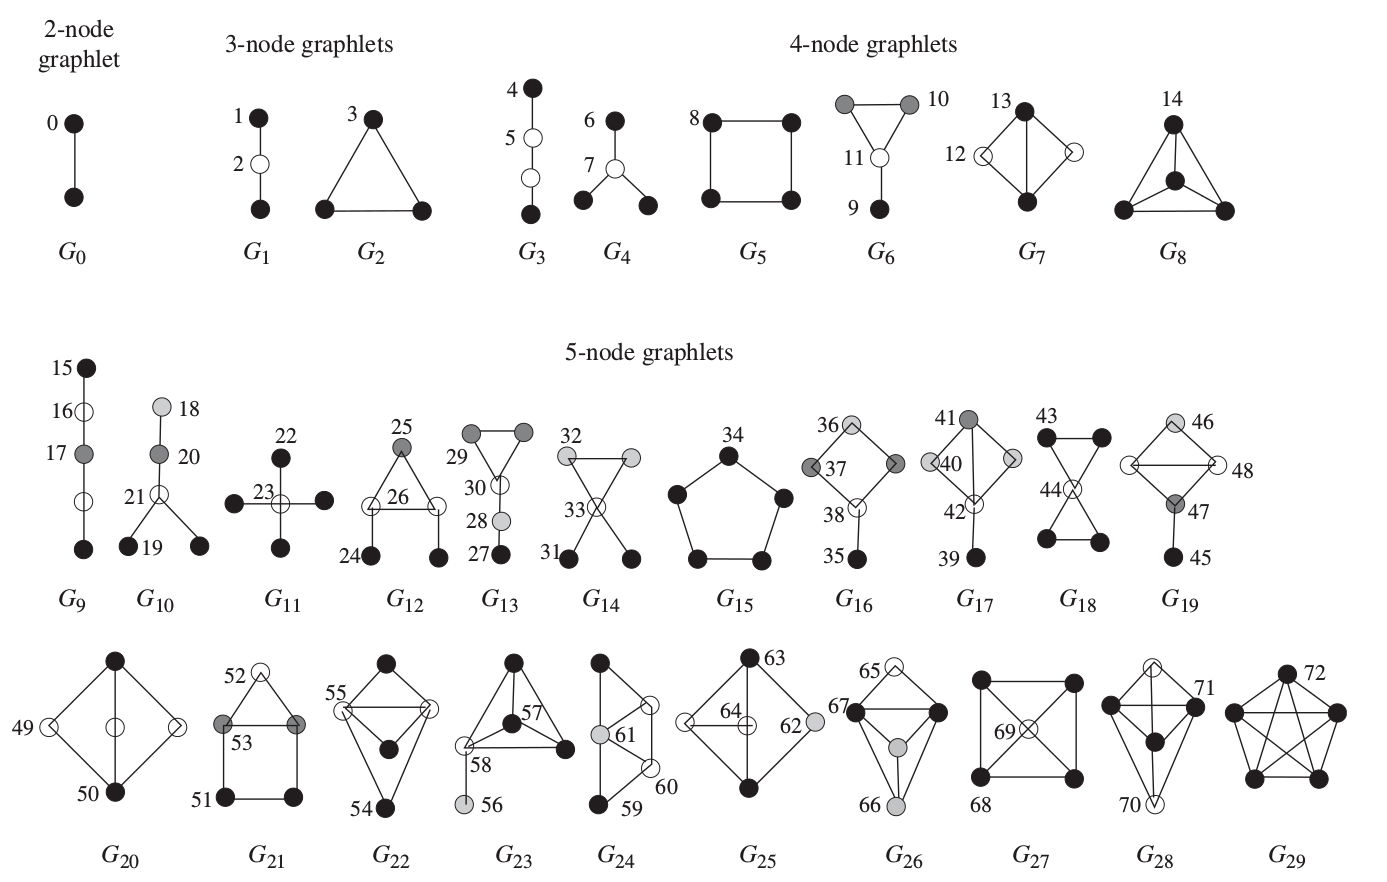
\includegraphics[width=\textwidth]{pic/graphlet.png}
\captionsetup{margin=50pt}
\caption{所有点数小于等于5的互不同构的小图\cite{kuchaiev2010topological}}\label{fig:graphlet}
\end{figure}

\begin{figure}[htbp]
\centering
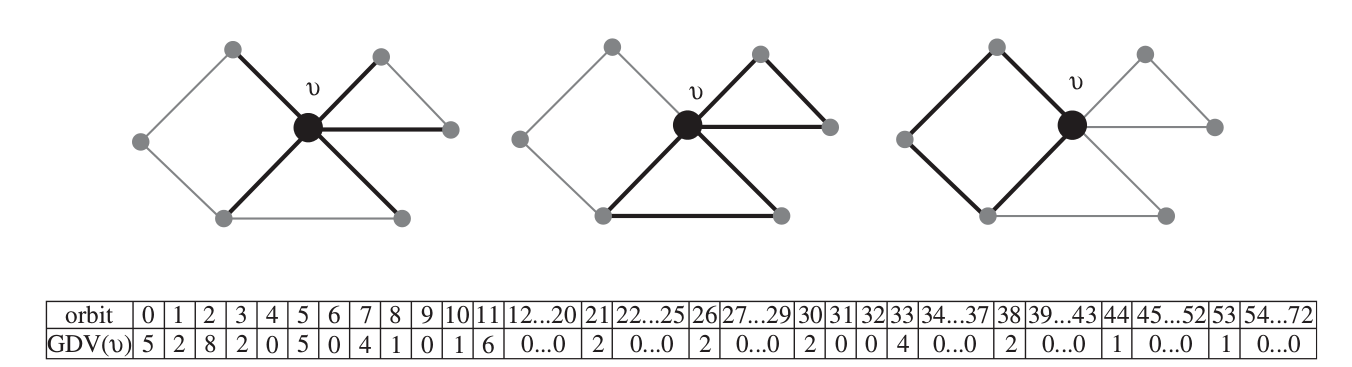
\includegraphics[width=\textwidth]{pic/orbitcount.png}
\captionsetup{margin=50pt}
\caption{点$v$的小图度数$GDV(v)\cite{kuchaiev2010topological}$}\label{fig:orbitcount}
\end{figure}

在由于小图度数这个衡量指标以后,类似于IsoRank,GRAAL也定义了两个点之间的相似度
\begin{equation}\label{graal1}
S(u,v)=1-\frac{\sum_{i=0}^{72}D_i(u,v)}{\sum_{i=0}^{72}w_i}
\end{equation}
其中
\begin{equation}\label{graal1}
D_i(u,v)=\frac{w_i*\left | log(u_i+1)-log(v_i+1) \right |}{log(max\{u_i,v_i\}+2)}
\end{equation}
$u_i$和$v_i$分别是点$u$和点$v$的第$i$维向量值,$w_i$是和第$i$个orbit相关的一个权重。

在有了相似度函数以后,GRAAL也和IsoRank一样,通过相似度函数,设计了一种寻找匹配的策略,然而不同于IsoRank的策略,GRALL采取的策略是,每次挑选出一个还没匹配过的点对$(i,j)$,称为种子点对(seed pair),然后将i的邻居点集和j的邻居点集根据相似度进行贪心的匹配,当i和j的邻居都不可再匹配的时候,GRAAL才继续寻找下一个种子点对,这是和IsoRank不同的地方。
GRAAL系列之后又出现了H-GRAAL\cite{milenkovic2010optimal},MI-GRAAL\cite{kuchaiev2011integrative},C-GRAAL\cite{memivsevic2012c}和L-GRAAL\cite{malod2015graal}。而最近提出的L-GRAAL\cite{malod2015graal}算法,通过解线性规划的问题来进行匹配,显示出了极好的匹配效果。

%@@@@@@@@@@@@@@@@@@@@@@@@@@@@@@@@@@@@@@@@@@@@@@@@@@@@@@@@@@@@@@@@@@@@@@
\subsection{SPINAL算法}
SPINAL算法(scalable protein interaction network alignment)也是类似于IsoRank和GRAAL的分两步算法。第一步,定义节点之间的相似度$P_{ij}$,并且与IsoRank类似的,它采用不断迭代的方式不断更新$P$的值,$P$的初始值由两个节点之间的度数差决定

\begin{equation}\label{spinal1}
P(i,j)=DegDiff(i,j)
\end{equation}

定义$NBG(\left \{ \left \langle i,j \right \rangle \right \},P)$为一个二分图,其中二分图左边的顶点集合由点$i$的邻居集合$N(i)$构成,右边的顶点集合由点$j$的邻居集合$N(j)$构成,边权则是它们对应的$P$值。
每一轮迭代,对于任意点对$(i,j)$,SPINAL算法对$NBG(\left \{ \left \langle i,j \right \rangle \right \},P)$进行二分图最大权匹配,令得到的匹配边集合为$C$,称为贡献者集合(contributors set),则新的$P$值为

\begin{equation}\label{spinal2}
P(i,j)=\frac{\sum_{(x_i,y_j)\in C}\frac{P(x_i,y_j)}{deg(x_i)*deg(y_j)}}{\sqrt{\left | C \right |}}
\end{equation}
通过若干论迭代,得到最后的相似度矩阵$P$。

SPINAL算法的第二步也是根据$P$矩阵对点对进行匹配的过程,和GRAAL算法类似,每一次,算法先找出当前$P$值最大的还未得到匹配的种子点对$(i,j)$,然后构造出由$i,j$的邻居集合构成的二分图,求出二分图的最大权值匹配边集合$M$。之后,SPINAL会重新依次检查二分图中的每一条非匹配边(不在集合$M$中),看看是否能够通过交换这条非匹配边与$M$中的匹配边得到更优的匹配。这相当于是一个局部调优的过程。然后再去寻找新的种子点对,进行下一轮的局部调优过程。
%@@@@@@@@@@@@@@@@@@@@@@@@@@@@@@@@@@@@@@@@@@@@@@@@@@@@@@@@@@@@@@@@@@@@
\subsection{PROPER算法}
PROPER算法(PROtein-protein interaction network alignment based on PERcolatin)\cite{kazemi2016proper}是一种基于图渗透的全局匹配算法。对于两个待匹配的图,PROPER算法用点对间的BLAST分数\cite{altschul1990basic}(一种衡量蛋白质序列之间相似度的分数)作为两个图任意点对之间的相似度函数

\begin{equation}\label{proper1}
S(i,j)=BLAST\_SCORE(i,j)
\end{equation}

与其他算法不同的是,在计算相似度的时候,PROPER算法并没有考虑点对之间的网络拓扑结构相似度,而只是单纯用了蛋白质序列的相似度。算法本身也是分两步走,第一步,算法按照相似度从大到小对所有点对进行排序。然后依次考虑每一点对$S(i,j)\geq l$,直到找到i和j都没有被匹配过的点对,将$(i,j)$加入集合$A$。最后的集合$A$就是第一步产生的部分匹配结果。

PROPER算法的第二步是在第一步结果$A$的基础上,扩展匹配的过程(图渗透算法)。定义

\begin{equation}\label{proper2}
F_A(i,j)=\left | \{(u,v):u\in N(i),v\in N(j),(u,v)\in A\} \right |
\end{equation}
称为点对$(i,j)$在已有匹配$A$下的贡献值,可以看到该值的实际意义就是,源网络在已有匹配$A$的情况下,通过匹配点对$(i,j)$能够增加的被匹配的边数。而匹配的衡量标准告诉我们被匹配的边数越多,则说明该匹配更好。因此,PROPER算法的第二步,便是将所有$F_A\geq r$且没有被匹配过的点对,按照$F_A$的值进行排序,挑选其中最好的一对加入集合$A$的过程。在集合$A$变化了以后,所有点对的$F_A$值重新计算,重新排序,重新挑选。

可以看到阈值$l$和$r$对PROPER算法有着极为重要的意义和影响。阈值$l$越小,第一步中被加入$A$的点对就越多,而阈值$r$越大,第二部中能够增加匹配的点对就越少。因此$l$和$r$分别控制了蛋白质序列相似度和网络结构相似度对整个算法的影响比例。

%@@@@@@@@@@@@@@@@@@@@@@@@@@@@@@@@@@@@@@@@@@@@@@@@@@@@@@@@@@@@@@@@@@@
\subsection{动态PPI网络生成}
本来,所有的PPI网络数据都是静态的,如何将PPI网络构造成动态的呢?\cite{zhang2016method}给出了一种合理的动态PPI网络构造方法。

基因表达数据(gene expression data)是对一个蛋白质在生物细胞作用中表现出来的基因水平提供衡量指标的数据。通过基因表达数据,我们可以很容易的直到生物体中的每一个蛋白质,在细胞生命活动的各个阶段,所表现出来的基因表达水平(gene expression level)分别是多少,可以知道,当蛋白质完成它在细胞活动中的作用是,其基因表达水平会明显下降,反之,则会处于高度活跃状态。因此,一个简单的想法就是,通过查看一个蛋白质的各个时刻的基因表达水平,来判断它在哪些时刻是处于活跃状态,那些时刻是处于不活跃状态的。定义一个蛋白质的基因表达数据为

\begin{equation}\label{dppi1}
p=[ p_1,p_2,p_3,....,p_n]
\end{equation}
$p$是一个数值序列,其中$p_i$为该蛋白质在$i$时刻的基因表达水平。\cite{zhang2016method}使用了一种三-西格玛阈值的方法来确定一个蛋白质何时处于活跃阶段,何时处于不活跃阶段。定义

\begin{equation}\label{dppi2}
Thresh_k(p)=\alpha (p)+k*\sigma (p)*\left (1-\frac{1}{1+\sigma ^2(p)}\right )
\end{equation}
为该蛋白质基因表达数据的三-西格玛阈值($k=1,2,3$)。其中$\alpha (p)$为$p$序列的平均值,$\sigma (p)$为标准差。

如果把$p$序列看成一个服从正态分布$N(\alpha,\sigma)$的随机变量,那么可以知道,$P(|X-\alpha|<\sigma)\approx 0.6827,P(|X-\alpha|<2\sigma)\approx 0.9545,P(|X-\alpha|<3\sigma)\approx 0.9973$。定义

\begin{equation}\label{dppi3}
Pr_i(p)= \begin{cases}
0.99 & \text{  } p_i\geq Thresh_3(p)\\ 
0.95 & \text{  } Thresh_3(p)> p_i\geq Thresh_2(p) \\ 
0.68 & \text{  } Thresh_2(p)> p_i\geq Thresh_1(p) \\ 
0 & \text{  } p_i<Thresh_1(p) 
\end{cases}
\end{equation}


为蛋白质在$i$时刻活跃的概率。那么

\begin{equation}\label{dppi4}
Pr_i((u,v))= Pr_i(u)*Pr_i(v)
\end{equation}
就是边$(u,v)$在$i$时刻活跃的概率。这样,一个静态的PPI网络就变成了由$n$个静态网络组成的动态PPI网络,其中每个蛋白质及蛋白质相互之间的作用在每个网络中都不同。